\section*{Chapitre 3}
\section{Conception Préliminaire}

\indent Cette étape nous permet, à partir des différents éléments de l'analyse, de mettre en forme les fonctions et procédures afin d'en expliciter les nouveaux fonctionnements.

\subsection{Diagramme de cas d'utilisation}

\begin{figure}[ht]
\centering
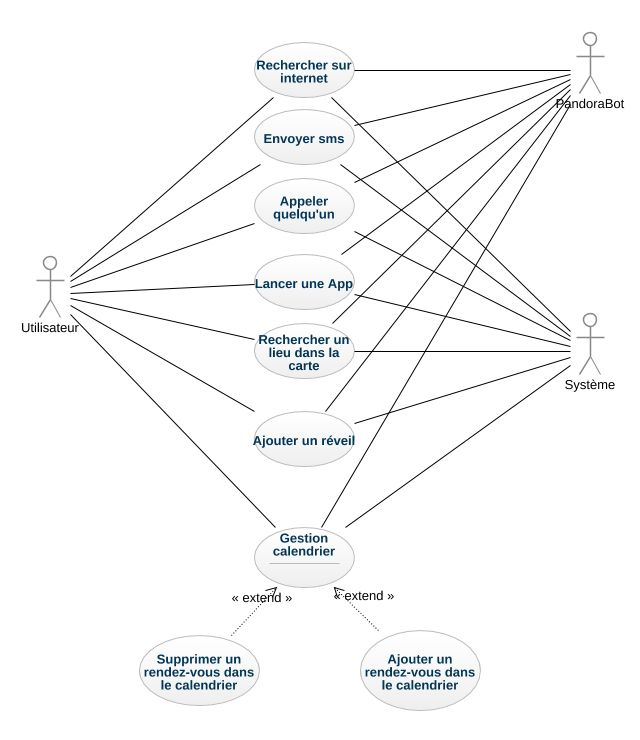
\includegraphics[scale=0.5]{./diagrammes/UsecaseDiagram.jpeg}
\caption{Diagramme de cas d'utilisation.\label{fig2}}
\end{figure}

\indent La F\begin{footnotesize}IGURE\end{footnotesize} \ref{fig2} représente le diagramme de cas d'utilisation pour les fonctionnalités déjà existantes et celles que nous souhaitons à réaliser. Les fonctionnalités déjà existantes sont : Rechercher sur Internet, Appeler quelqu'un et Lancer une App. La gestion calendrier est modifiée par nous. Le reste est les fonctionnalités ajoutées par nous.

\subsection{Diagramme de Sequence}

\begin{figure}[ht]
\centering
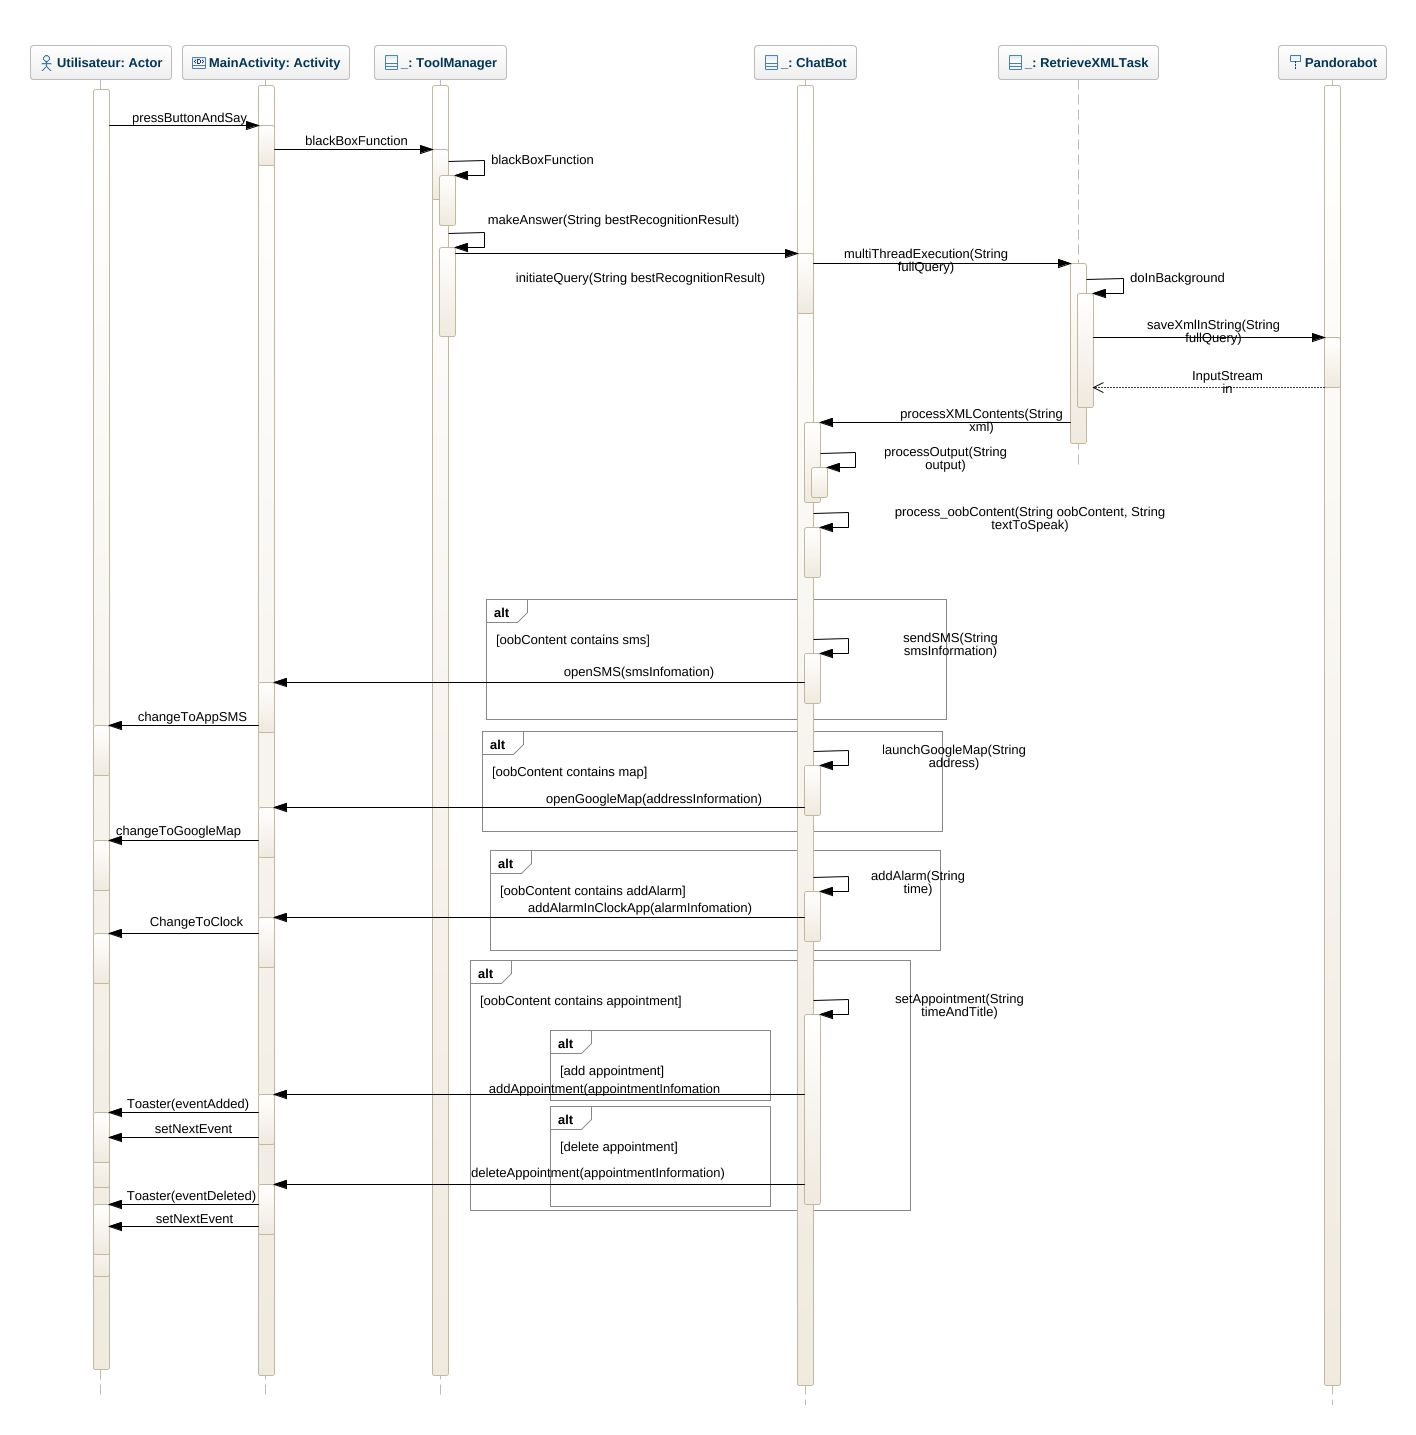
\includegraphics[scale=0.4]{./diagrammes/SequenceDiagram.jpeg}
\caption{Diagramme de Sequence.\label{fig3}}
\end{figure}

\indent La F\begin{footnotesize}IGURE\end{footnotesize} \ref{fig3} représente un diagramme de séquence pour les fonctionnalités que nous avons proposé de réaliser. Les parties <<boite noire>> sont les parties du code qui ont été complétées dans les dernières versions. Ce que nous avons construit est la partie au-dessous de \textbf{\emph{process$_-$oobContent(String oobContent, String textToSpeak)}}.
\newpage

\subsection{Signatures Partie Chatbot}

\indent Dans cette section, \textbf{\emph{oobContent}} est une chaîne de caractères retournée par Pandorabots qui contient une étiquette \textbf{\emph{<oob>}} et des informations de la réponse intélligente.

\indent Classe \textbf{\emph{GestionCalendar}} est le module de gestion des fonctions liées au traitement du calendrier.\\

\indent procédure setAppointement (E/S Gcal : GestionCalendar, E oobContent : String, operationType : String)\\
\indent fonction setBeginTimeAndGetTitle (E oobContent : String, beginTime : Calendar, operationType : String) : String\\
\indent procédure googleQuery (E/S googleSearchText : String)\\
\indent procédure launchApp (E app : String)\\
\indent procédure launchUrl (E/S url : String)\\
\indent procédure launchGoogleMap (E/S address : String)\\
\indent procédure sendSMS (E oobContent : String)\\
\indent procédure makePhoneCall (E oobContent : String)\\
\indent procédure addAnAlarm(E oobContent : String)\\
\indent procédure deleteAnAlarm (E oobContent : String)\\

\subsection{Signatures Partie ToolManager}

\indent procédure setNextEvent()\\
\indent fonction getNextEvent() : String\\
\newpage

